% Plantilla para documentos LaTeX para enunciados
% Por Pedro Pablo Aste Kompen - ppaste@uc.cl
% Licencia Creative Commons BY-NC-SA 3.0
% http://creativecommons.org/licenses/by-nc-sa/3.0/

\documentclass[12pt]{article}

% Margen de 1 pulgada por lado
\usepackage{fullpage}
% Incluye gráficas
\usepackage{graphicx}
% Packages para matemáticas, por la American Mathematical Society
\usepackage{amssymb}
\usepackage{amsmath}
% Desactivar hyphenation
\usepackage[none]{hyphenat}
% Saltar entre párrafos - sin sangrías
\usepackage{parskip}
% Español y UTF-8
\usepackage[spanish]{babel}
\usepackage[utf8]{inputenc}
% Links en el documento
\usepackage{hyperref}
\usepackage{fancyhdr}
\setlength{\headheight}{15.2pt}
\setlength{\headsep}{5pt}
\pagestyle{fancy}

\newcommand{\N}{\mathbb{N}}
\newcommand{\Exp}[1]{\mathcal{E}_{#1}}
\newcommand{\List}[1]{\mathcal{L}_{#1}}
\newcommand{\EN}{\Exp{\N}}
\newcommand{\LN}{\List{\N}}

\newcommand{\comment}[1]{}
\newcommand{\lb}{\\~\\}
\newcommand{\eop}{_{\square}}
\newcommand{\hsig}{\hat{\sigma}}
\newcommand{\ra}{\rightarrow}
\newcommand{\lra}{\leftrightarrow}

% Cambiar por nombre completo + número de alumno
\newcommand{\alumno}{Matias Araos, Vicente Rivas, Victor Ruiz - Grupo 15}
\rhead{Entrega 2 - \alumno}

\begin{document}
\thispagestyle{empty}
% Membrete
% PUC-ING-DCC-IIC1103
\begin{minipage}{2.3cm}

\includegraphics[width=2cm]{img/logo.pdf}
\vspace{0.5cm} % Altura de la corona del logo, así el texto queda alineado verticalmente con el círculo del logo.
\end{minipage}
\begin{minipage}{\linewidth}
\textsc{\raggedright \footnotesize
Pontificia Universidad Católica de Chile \\
Departamento de Ciencia de la Computación \\
IIC2413 - Bases de Datos \\}
\end{minipage}


% Titulo
\begin{center}
\vspace{0.5cm}
{\huge\bf Entrega 2}\\
\vspace{0.2cm}
\today\\
\vspace{0.2cm}
\footnotesize{2º semestre 2024 - Profesores Eduardo Bustos  - Christian Alvarez}\\
\vspace{0.2cm}
\footnotesize{\alumno}
\rule{\textwidth}{0.05mm}
\end{center}



\section*{Diagrama E/R}
\begin{center}
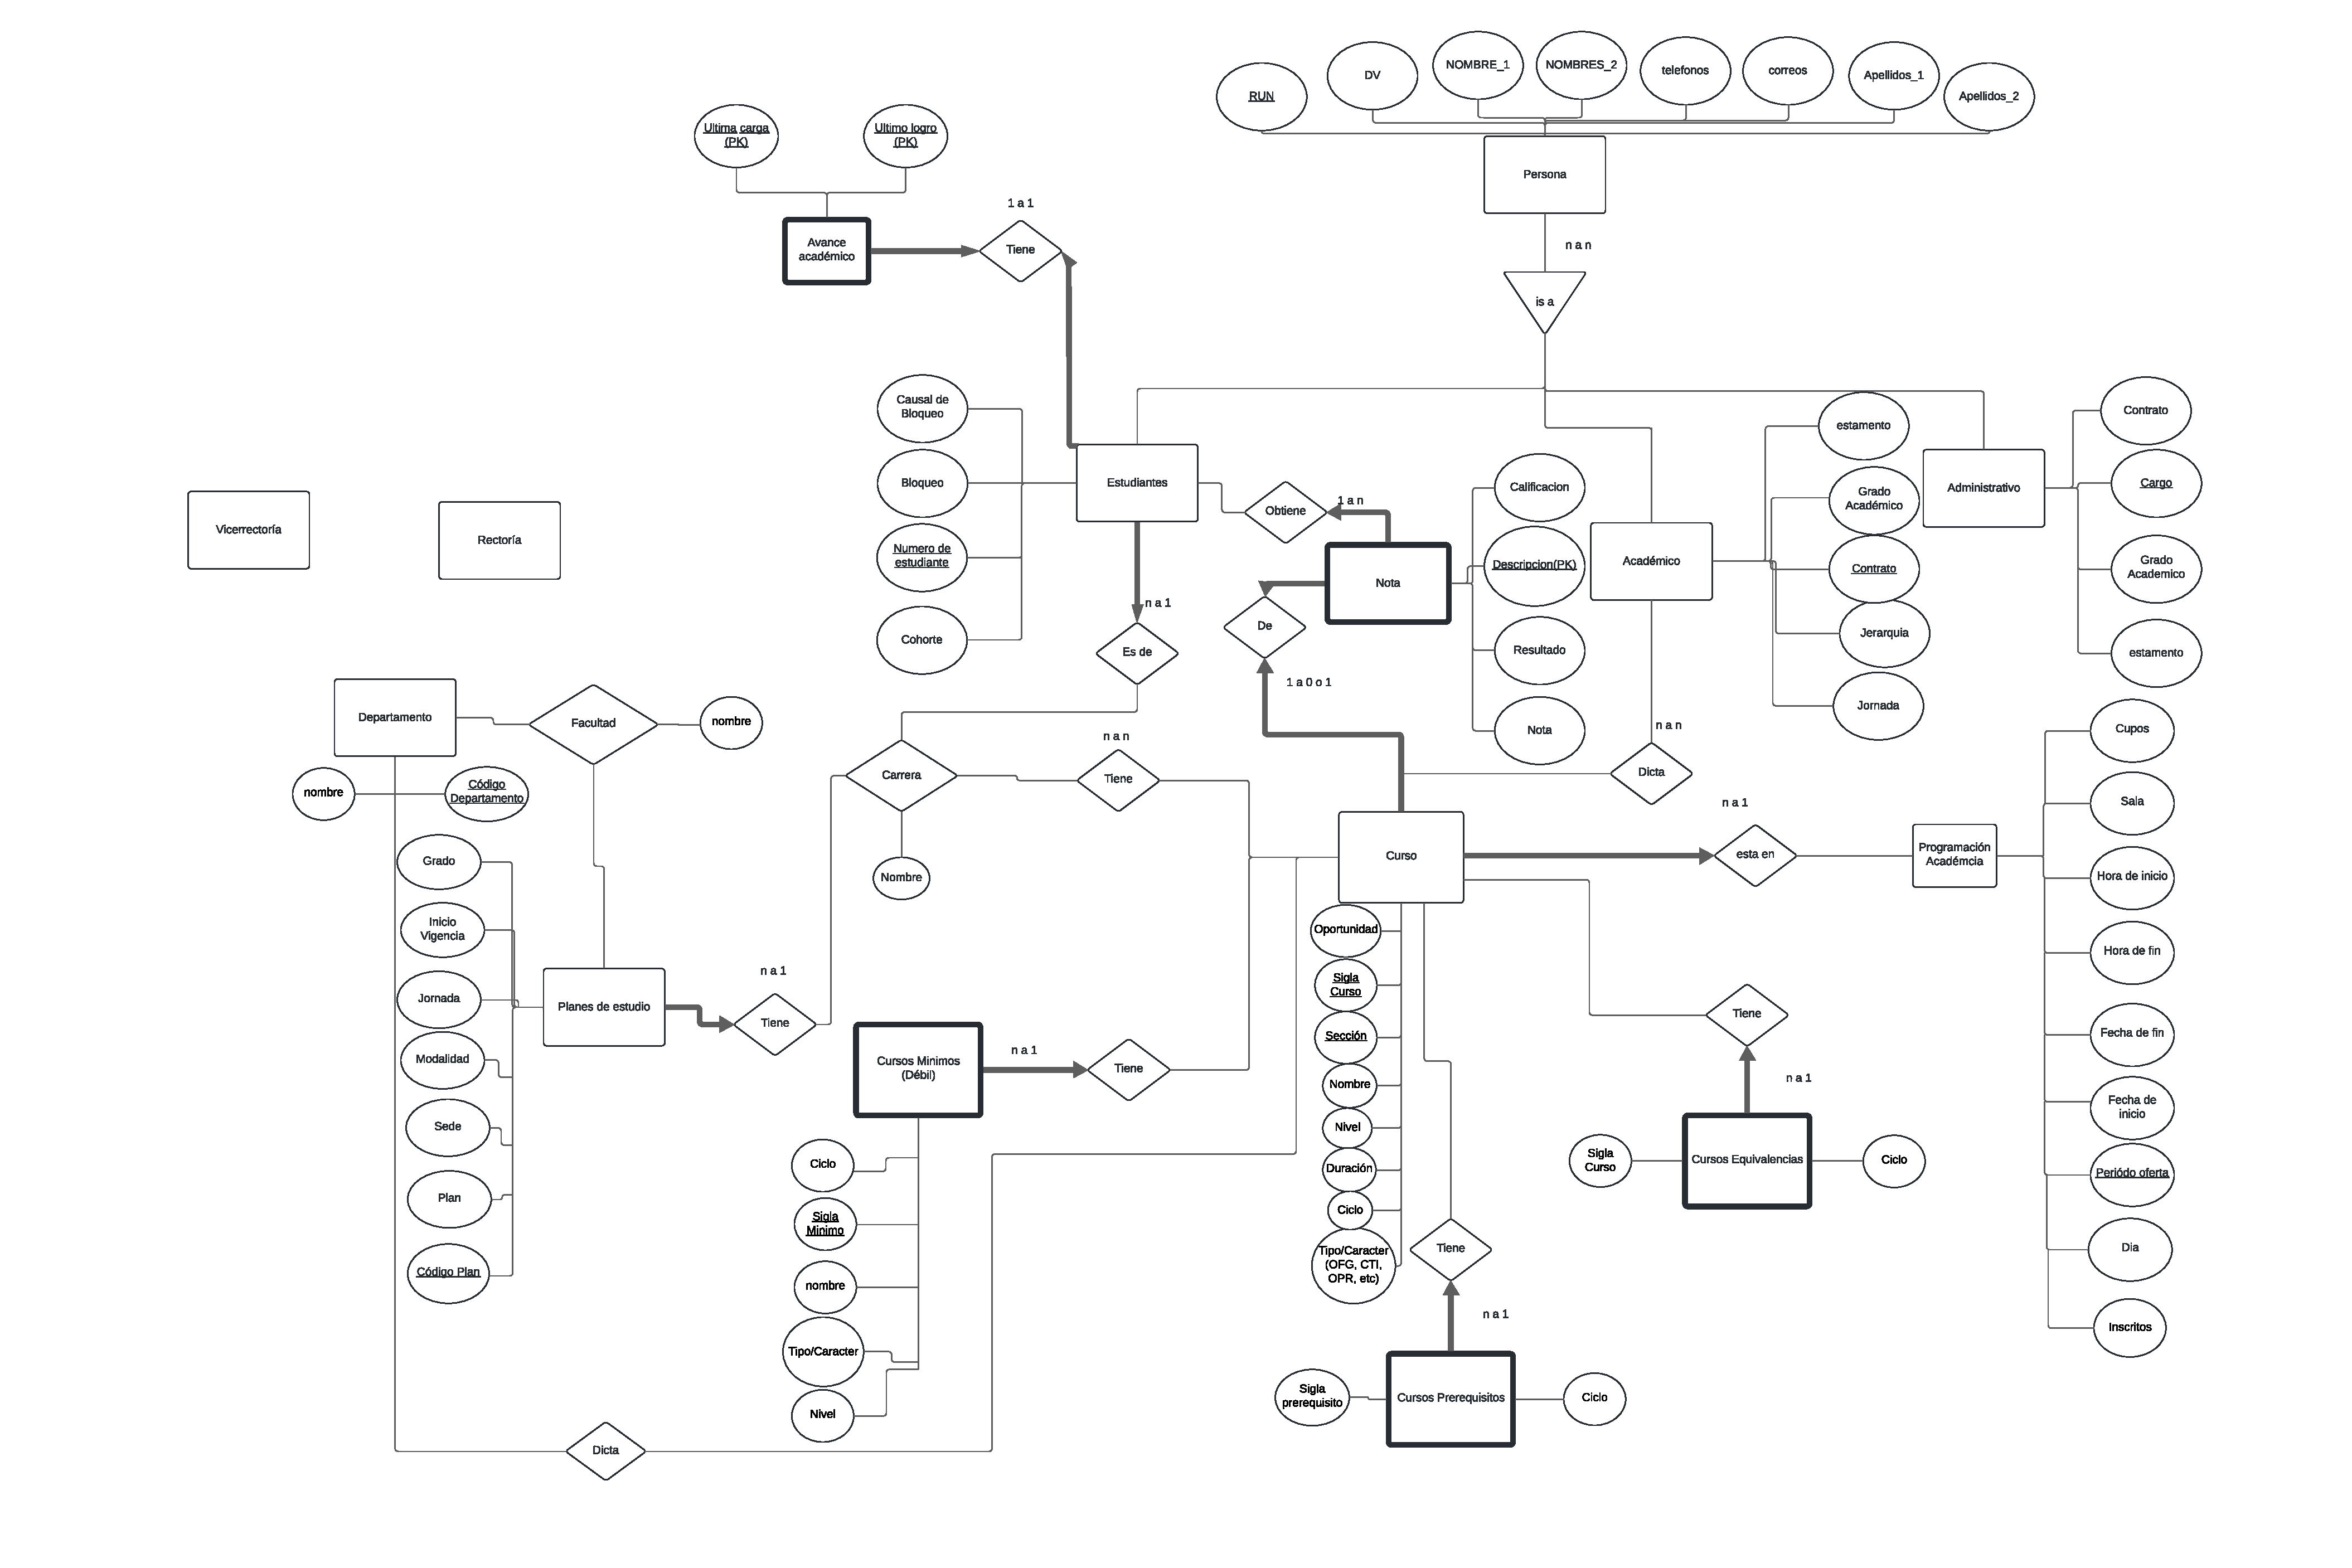
\includegraphics[width=1.1\textwidth]{img/Diagrama_er_1.pdf}
\end{center}

\section*{Esquema Relacional}
\textit{Persona}(\underline{RUT}: int, \underline{DV}: int, Nombres: string, Apellido\_Paterno: string, Apellido\_Materno: string, Nombre\_Completo: string, Mail\_Personal: string, Mail\_Institucional: string, Teléfono: string) \\\\
\textit{Estudiante}(\underline{Persona.RUT}: int, \underline{Persona.DV}: int, \underline{Número\_de\_Estudiante}: int, Carrera: string, Cohorte: string, Estado: string, Bloqueo: bool) \\\\
\textit{Académico}(\underline{Persona.RUT}: int, \underline{Persona.DV}: int, Contrato: string, Jerarquía: string, Jornada: string, Grado\_Académico: string) \\\\
\textit{Administrativo}(\underline{Persona.RUT}: int, \underline{Persona.DV}: int, Cargo: string, Grado\_Académico: string) \\\\
\textit{Curso}(\underline{Sigla\_Curso}: string, \underline{Sección}: int, Nombre: string, Nivel: string, Tipo/Carácter (OFG, CTI, OPR, etc.): string, Ciclo: int, Departamento.Código\_Departamento: string) \\\\
\textit{Cursos\_Equivalencias}(\underline{Curso.Sigla\_Curso}: string, \underline{Curso.Sección}: int, Sigla\_Equivalente: string, Ciclo: int) \\\\
\textit{Cursos\_Prerequisitos}(\underline{Curso.Sigla\_Curso}: string, \underline{Curso.Sección}: int, Sigla\_Prerequisito: string, Ciclo: int) \\\\
\textit{Cursos\_Minimos}(\underline{Curso.Sigla\_Curso}: string, \underline{Curso.Sección}: int, Curso\_Minimo: string, Ciclo: int) \\\\
\textit{Planes\_Estudio}(\underline{Código\_Plan}: string, Nombre: string, Facultad: string, Nivel: string, Modalidad: string, Fecha\_Inicio: string) \\\\
\textit{Programacion\_Academica}(\underline{Curso.Sigla\_Curso}: string, \underline{Curso.Sección}: int, Periodo: string, Sala: string, Horario: string, Vacantes: int) \\\\
\textit{Departamento}(\underline{Código\_Departamento}: string, Nombre: string, Facultad: string) \\\\
\textit{Nota}(\underline{Curso.Sigla\_Curso}: string, \underline{Curso.Sección}: int, \underline{Estudiante.Número\_de\_Estudiante}: int, Ciclo: int, Nota: float, Descripción: string, Calificación: string, Resultado: string) \\\\
\textit{Avance\_Academico}(\underline{Estudiante.Número\_de\_Estudiante}: int, \underline{Curso.Sigla\_Curso}: string, \underline{Curso.Sección}: int, Última\_Carga: string, Último\_Logro: string)

\subsection*{Restricciones de Integridad y Dominios}
% Aca avisamos con un disclaimer que si en el dominio existe nulo entonces admite nulo, si no, se asume que no admite nulo, lo ponemos en mayúscula para que se note
% Ponemos en mayúscula el aviso:
\textbf{Nota:} Si en el dominio existe nulo entonces admite nulo, si no, se asume que no admite nulo.\\\\

\textit{Nota.Calificacion} $\in$ \{SO, MB, B, SU, I, M, MM, NP, EX, A, R, nulo\}\\\\
\textit{Prerrequisito.Ciclo} $\in$ \{B, L\}\\\\
\textit{Estudiante.Bloqueo} $\in$ \{S, N\}\\\\
\textit{Academico.Jornada} $\in$ \{Completa, Diurna, Vespertina\}\\\\
\textit{Programacion\_Academica.Modulo\_Horario} $\in$ \{1, 2, 3, 4, 5, 6, 7, 8, 9\}\\\\
\textit{Persona.DV} $\in$ \{0, 1, 2, 3, 4, 5, 6, 7, 8, 9, K\}\\\\
% Curso.Nivel tiene dos dominios, 1...10 o B, L, lo agregamos con una disyunción
\textit{Curso.Nivel} $\in$ \{1, 2, 3, 4, 5, 6, 7, 8, 9, 10\} $\cup$ \{B, L\}\\\\
\textit{Nota.Descripcion} $\in$ \{Sobresaliente, Muy Bueno, Bueno, Suficiente, Insuficiente, Malo, Muy Malo, Nota Pendiente, Eximido, Aprobado, Reprobado, curso vigente\}\\\\
\textit{Nota.Nota} $\in$ \{1.0 - 1.9, 2.0 - 2.9, 3.0 - 3.9, 4.0 - 4.9, 5.0 - 5.9, 6.0 - 6.5, 6.6 - 7.0, nulo\}\\\\
\textit{Nota.Resultado} $\in$ \{Aprobatorio, Reprobatorio, Curso incompleto, Curso Vigente en el período académico\}\\\\
\textit{Avance\_Academico.Ultimo\_Logro} $\in$ \{Ingreso, 1...10, Licenciatura\}\\\\
\textit{Avance\_Academico.Ultima\_Carga} $\in$ \{año-semestre\}\\\\
\textit{Estudiante.Cohorte} $\in$ \{año-semestre\}\\\\
\textit{Programacion\_Academica.Periodo\_Oferta} $\in$ \{año-semestre\}\\\\

% Nuevos dominios y restricciones de integridad basados en las tablas proporcionadas
\textit{Persona.Nombre\_1, Persona.Nombre\_2, Persona.Apellido\_1, Persona.Apellido\_2} $\in$ \{Cadenas de caracteres\}\\\\
\textit{Persona.Correos, Persona.Telefonos} $\in$ \{Cadenas de caracteres\}\\\\
\textit{Estudiante.Causal\_de\_bloqueo} $\in$ \{Texto\}\\\\
\textit{Estudiante.Nombre\_Carrera} $\in$ \{Cadenas de caracteres\}\\\\
\textit{Academico.Estamento, Academico.Grado\_academico, Academico.Contrato, Academico.Jerarquia} $\in$ \{Cadenas de caracteres\}\\\\
\textit{Administrativo.Estamento, Administrativo.Grado\_academico, Administrativo.Contrato, Administrativo.Cargo} $\in$ \{Cadenas de caracteres\}\\\\
\textit{Curso.Nombre, Curso.Tipo, Curso.Oportunidad, Curso.Duracion, Curso.Nombre\_Departamento, Curso.Codigo\_Departamento, Curso.RUN\_Academico, Curso.DV\_Academico, Curso.Nombre\_Academico, Curso.Apellido1\_Academico, Curso.Apellido2\_Academico, Curso.Principal, Curso.Plan\_curso} $\in$ \{Cadenas de caracteres\}\\\\
\textit{Curso.Seccion\_curso} $\in$ \{Enteros\}\\\\
\textit{Curso.Periodo\_curso} $\in$ \{año-semestre\}\\\\
\textit{Curso\_Equivalencias.Sigla\_equivalente} $\in$ \{Cadenas de caracteres\}\\\\
\textit{Curso\_Minimos.Sigla\_minimo, Curso\_Minimos.Nombre, Curso\_Minimos.Tipo, Curso\_Minimos.Nivel} $\in$ \{Cadenas de caracteres\}\\\\
\textit{Planes\_Estudio.Codigo\_Plan, Planes\_Estudio.Jornada, Planes\_Estudio.Modalidad, Planes\_Estudio.Sede, Planes\_Estudio.Plan, Planes\_Estudio.Nombre\_Facultad, Planes\_Estudio.Grado, Planes\_Estudio.Nombre\_Carrera} $\in$ \{Cadenas de caracteres\}\\\\
\textit{Planes\_Estudio.Inicio\_Vigencia} $\in$ \{Fecha\}\\\\
\textit{Programacion\_Academica.Sigla\_curso, Programacion\_Academica.Sala} $\in$ \{Cadenas de caracteres\}\\\\
\textit{Programacion\_Academica.Seccion\_curso, Programacion\_Academica.Cupos, Programacion\_Academica.Inscritos} $\in$ \{Enteros\}\\\\
\textit{Programacion\_Academica.Hora\_Inicio, Programacion\_Academica.Hora\_Fin} $\in$ \{Hora\}\\\\
\textit{Programacion\_Academica.Fecha\_Inicio, Programacion\_Academica.Fecha\_Fin} $\in$ \{Fecha\}\\\\
\textit{Departamento.Nombre, Departamento.Codigo, Departamento.Nombre\_Facultad} $\in$ \{Cadenas de caracteres\}\\\\
\textit{Nota.Numero\_de\_estudiante} $\in$ \{Enteros\}\\\\
\textit{Nota.Descripcion} $\in$ \{Cadenas de caracteres\}\\\\
\textit{Nota.Nota} $\in$ \{1.0 - 7.0\}\\\\
\textit{Nota.Calificacion} $\in$ \{Cadenas de caracteres\}\\\\
\textit{Avance\_Academico.Periodo\_Oferta, Avance\_Academico.Descripcion, Avance\_Academico.Resultado, Avance\_Academico.Calificacion, Avance\_Academico.Ultima\_Carga, Avance\_Academico.Ultimo\_Logro, Avance\_Academico.Fecha\_logro} $\in$ \{Cadenas de caracteres\}\\\\
\textit{Avance\_Academico.Nota} $\in$ \{1.0 - 7.0\}\\\\


\section*{Estrategias para el Manejo de Violaciones a las Restricciones de Integridad y Formato}

\subsection*{Validación de Datos}
Se desarrollaron funciones específicas para verificar la integridad de los datos antes de su inserción en la base de datos.

\subsection*{Corrección de Datos}
Para mantener la uniformidad en los datos, se implementaron mecanismos de corrección automática, para ajustar formato, convertir codificación o corregir otros errores, para así evitar problemas y restricciones de integridad.

\subsection*{Manejo de Duplicados}
Para prevenir la inserción de registros duplicados en la base de datos, se utilizó la cláusula \texttt{ON CONFLICT DO NOTHING} en las consultas de inserción. Esta estrategia permite que el sistema ignore intentos de insertar registros que ya existen basándose en las claves únicas definidas, manteniendo así la integridad de los datos sin interrumpir el flujo de procesamiento.

\subsection*{Registro de Errores}
Cuando se detectan inconsistencias o errores durante la inserción de datos, el sistema registra automáticamente estos incidentes en archivos CSV específicos mediante la función \texttt{registrarError}. Este enfoque permite identificar y analizar los registros problemáticos posteriormente, facilitando la depuración y corrección de datos sin detener la ejecución del script.

\subsection*{Creación de Triggers}
Se desarrollaron triggers en la base de datos para automatizar la actualización y validación de ciertos campos antes de realizar operaciones de actualización en las tablas principales.


\section*{Supuestos}

\subsection*{Formato de los Archivos CSV}
Se asume que los archivos CSV utilizados como fuentes de datos tienen un orden de columnas específicos que coinciden con los índices utilizados en el código PHP.

\subsection*{Ubicación de los Archivos}
Se asume que están en la carpeta \textit{data}.

\subsection*{Calidad de los Valores Obtenidos}
Se espera que no todos sean perfectos, por lo mismo, se corrigen con el código. Por ejemplo, se asume que Nota puede ser NULL en los datos que se entregan al código, que luego este procede a corregir. 

\subsection*{Nombre-Apellido}
Los nombres y apellidos solo contienen letras del alfabeto castellano, guiones, espacios y apóstrofes.

\subsection*{Correos}
Los correos electrónicos cumplen con la norma IETF RFC 3696.

\subsection*{Fechas Examenes}
Los periodos de los examenes definidos se llevan a cabo unicamente en los periodos de Julio y Diciembre, ya que estos son los únicos periodos relevantes para la consulta de notas, por lo que son bastante relevantes para el analisis academico según las notas obtenidas en esos periodos.

\subsection*{Formato de Fechas Consistente}
Se asume que las fechas en los archivos CSV están en el formato \texttt{d/m/y} usado en este país.

\subsection*{Docentes y Academicos}
Se asume que dentro de la tabla de Docentes Planificados, todos aquellos con contrato, son considerados como Académico. Además, si la jerarqueria contiene la palabra "Docente", entonces el individuo ES "Docente" por virtud de su clasificación como tal.  

\subsection*{Grandes Cantidades de Datos}
Las consultas SQL están optimizadas para manejar grandes volúmenes de datos, aprovechando índices y evitando operaciones costosas cuando sea posible, asumiendo que el servidor tiene suficiente RAM para soportar el procesamiento requerido.

% Instrucciones para uso de la aplicacion y el cargador de datos

\section*{Instrucciones para el Cargador de Datos y la aplicacion Bananer}

Una vista general de la arquitectura de la aplicación Bananer es la siguiente:


\begin{center}
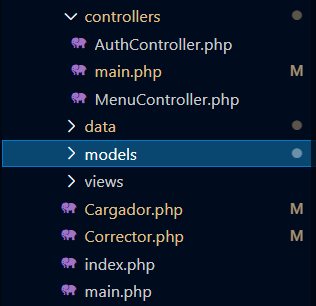
\includegraphics[width=0.5\textwidth]{img/arquitectura.png}
\end{center}

\subsection*{Instrucciones}
Para la correcta ejecución del programa, se debe correr \texttt{main.php} como se ve en la imagen. Se requiere PHP y PostgreSQL. Se deberá ingresar, en la terminal, para conectarse al servidor con \texttt{ssh grupo15@bdd1.ing.puc.cl}, con la contraseña \textit{Elefante\$15} e ingresar a PostgreSQL con los defaults. Luego, ir a \url{https://bdd1.ing.puc.cl/grupo15/index.php}.
Ahi, se deberá ingresar con las credenciales: Email: 'bananer@lamejor.com', y Clave: 'bananer0'. Se puede ejecutar también por terminal de comandos: host=localhost port=5432 dbname=grupo15 user=grupo15 \textit{Elefante\$15}

Si se quiere realizar la consulta para registrar nuevos usuarios se debera ingresar el correo de este usuario, junto a una clave cualquiera. 

% Fin del documento
\end{document}
